\documentclass[border=5pt]{standalone}
\usepackage[T1]{fontenc}
\usepackage{lmodern}
\usepackage{pgfplots}
\usepgfplotslibrary{groupplots}
\pgfplotsset{compat=1.18}
\begin{document}\sffamily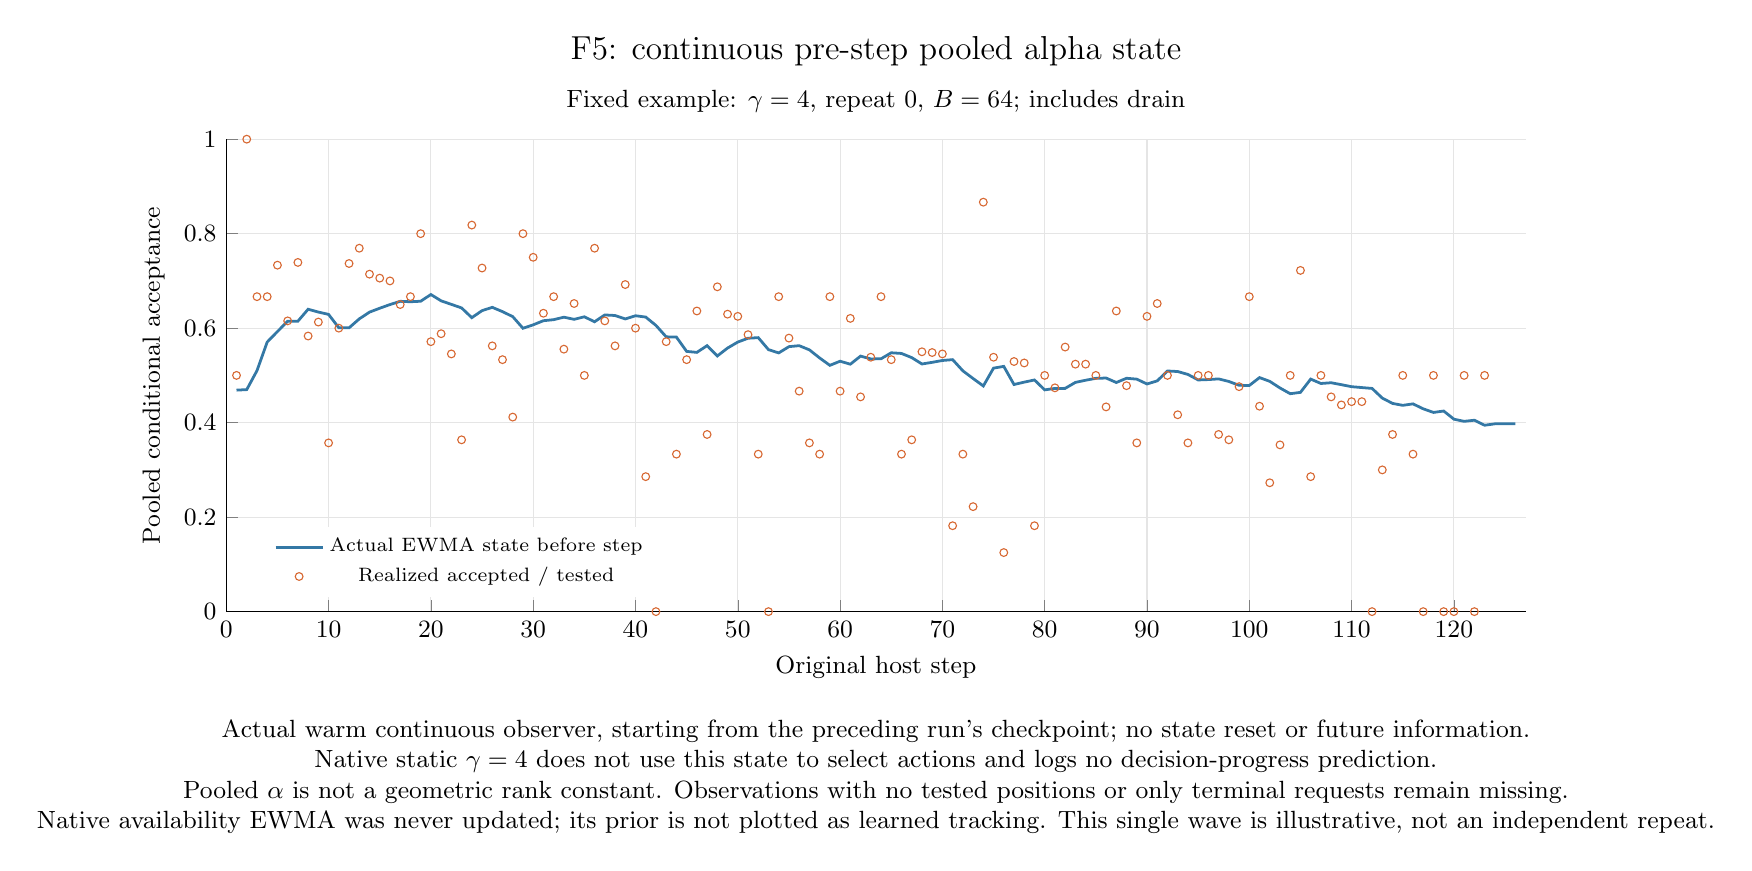
\begin{tikzpicture}
\definecolor{cal}{HTML}{3478A5}\definecolor{test}{HTML}{D76832}\definecolor{profile}{HTML}{3B8A5A}
\begin{groupplot}[group style={group size=1 by 1,horizontal sep=1.9cm},width=16.5cm,height=6.0cm,scale only axis,axis lines*=left,grid=major,grid style={gray!20},tick label style={font=\small},label style={font=\small},title style={font=\small},legend style={font=\scriptsize,draw=none},unbounded coords=jump]
\nextgroupplot[title={Fixed example: $\gamma=4$, repeat 0, $B=64$; includes drain},xlabel={Original host step},ylabel={Pooled conditional acceptance},xmin=0,xmax=127,ymin=0,ymax=1,legend pos=south west]
\addplot[color=cal,line width=1pt] coordinates {(1,0.46878656861) (2,0.46993685872) (3,0.510060113434) (4,0.570635783407) (5,0.592844781113) (6,0.614632054739) (7,0.614729838135) (8,0.64004011132) (9,0.63405738414) (10,0.629140280007) (11,0.600729043021) (12,0.600673232048) (13,0.619618193828) (14,0.633929074725) (15,0.64218183233) (16,0.64993431117) (17,0.656805946917) (18,0.655905363293) (19,0.656974149456) (20,0.671188825854) (21,0.657831049634) (22,0.65035006719) (23,0.642825097284) (24,0.6222142128) (25,0.637070232414) (26,0.644077877688) (27,0.634977832569) (28,0.624396449923) (29,0.599752849861) (30,0.607060467998) (31,0.615768902979) (32,0.617958656549) (33,0.623235333029) (34,0.618676611376) (35,0.624054722646) (36,0.613491549803) (37,0.627970005174) (38,0.626791703425) (39,0.619494493045) (40,0.626261979943) (41,0.623465840523) (42,0.605795079875) (43,0.581643570691) (44,0.581047069492) (45,0.550810204135) (46,0.548722964224) (47,0.563001112041) (48,0.541130081606) (49,0.557884291621) (50,0.570561571779) (51,0.578650364288) (52,0.5799071119) (53,0.554535560672) (54,0.547579516904) (55,0.560852722118) (56,0.562944635301) (57,0.554079897782) (58,0.536914480344) (59,0.521310255578) (60,0.530037304967) (61,0.523696536927) (62,0.540856010836) (63,0.53486710033) (64,0.535167260021) (65,0.547884106686) (66,0.546472302616) (67,0.537661138213) (68,0.524144565124) (69,0.527651297567) (70,0.531577680151) (71,0.533380466731) (72,0.509714869534) (73,0.493390160208) (74,0.477630869253) (75,0.515431776677) (76,0.519062072489) (77,0.480720845256) (78,0.485737491617) (79,0.490340408038) (80,0.469358967915) (81,0.472393205654) (82,0.47254239362) (83,0.485182556622) (84,0.489773767769) (85,0.49374437964) (86,0.494431775572) (87,0.484974217954) (88,0.493954999035) (89,0.492054030093) (90,0.481838807593) (91,0.48840558502) (92,0.509335495019) (93,0.508219108702) (94,0.502032172635) (95,0.490362016555) (96,0.491153713209) (97,0.492600837708) (98,0.487164260007) (99,0.479015304952) (100,0.478668541215) (101,0.495358283118) (102,0.487399998462) (103,0.473390839047) (104,0.461253416511) (105,0.464091395806) (106,0.492174349256) (107,0.482904528115) (108,0.484455485765) (109,0.480365449695) (110,0.476100110159) (111,0.474246684585) (112,0.472426321442) (113,0.45197642387) (114,0.440697932623) (115,0.436632277993) (116,0.439739894513) (117,0.429283270176) (118,0.421610698387) (119,0.424605208789) (120,0.407316654067) (121,0.402761336651) (122,0.405119378369) (123,0.394490044654) (124,0.397478825612) (125,0.397478825612) (126,0.397478825612)};
\addlegendentry{Actual EWMA state before step}
\addplot[only marks,color=test,mark=o,mark size=1.4pt] coordinates {(1,0.5) (2,1) (3,0.666666666667) (4,0.666666666667) (5,0.733333333333) (6,0.615384615385) (7,0.739130434783) (8,0.583333333333) (9,0.612903225806) (10,0.357142857143) (11,0.6) (12,0.736842105263) (13,0.769230769231) (14,0.714285714286) (15,0.705882352941) (16,0.7) (17,0.65) (18,0.666666666667) (19,0.8) (20,0.571428571429) (21,0.588235294118) (22,0.545454545455) (23,0.363636363636) (24,0.818181818182) (25,0.727272727273) (26,0.5625) (27,0.533333333333) (28,0.411764705882) (29,0.8) (30,0.75) (31,0.631578947368) (32,0.666666666667) (33,0.555555555556) (34,0.652173913043) (35,0.5) (36,0.769230769231) (37,0.615384615385) (38,0.5625) (39,0.692307692308) (40,0.6) (41,0.285714285714) (42,0) (43,0.571428571429) (44,0.333333333333) (45,0.533333333333) (46,0.636363636364) (47,0.375) (48,0.6875) (49,0.62962962963) (50,0.625) (51,0.586206896552) (52,0.333333333333) (53,0) (54,0.666666666667) (55,0.578947368421) (56,0.466666666667) (57,0.357142857143) (58,0.333333333333) (59,0.666666666667) (60,0.466666666667) (61,0.620689655172) (62,0.454545454545) (63,0.538461538462) (64,0.666666666667) (65,0.533333333333) (66,0.333333333333) (67,0.363636363636) (68,0.55) (69,0.548387096774) (70,0.545454545455) (71,0.181818181818) (72,0.333333333333) (73,0.222222222222) (74,0.866666666667) (75,0.538461538462) (76,0.125) (77,0.529411764706) (78,0.526315789474) (79,0.181818181818) (80,0.5) (81,0.473684210526) (82,0.56) (83,0.52380952381) (84,0.52380952381) (85,0.5) (86,0.433333333333) (87,0.636363636364) (88,0.478260869565) (89,0.357142857143) (90,0.625) (91,0.652173913043) (92,0.5) (93,0.416666666667) (94,0.357142857143) (95,0.5) (96,0.5) (97,0.375) (98,0.363636363636) (99,0.47619047619) (100,0.666666666667) (101,0.434782608696) (102,0.272727272727) (103,0.352941176471) (104,0.5) (105,0.722222222222) (106,0.285714285714) (107,0.5) (108,0.454545454545) (109,0.4375) (110,0.444444444444) (111,0.444444444444) (112,0) (113,0.3) (114,0.375) (115,0.5) (116,0.333333333333) (117,0) (118,0.5) (119,0) (120,0) (121,0.5) (122,0) (123,0.5)};
\addlegendentry{Realized accepted / tested}
\end{groupplot}
\path (group c1r1.north west) -- node[above=0.8cm,font=\large] {F5: continuous pre-step pooled alpha state} (group c1r1.north east);
\path (group c1r1.south west) -- node[below=1.25cm,align=center,font=\small] {Actual warm continuous observer, starting from the preceding run's checkpoint; no state reset or future information.\\Native static $\gamma=4$ does not use this state to select actions and logs no decision-progress prediction.\\Pooled $\alpha$ is not a geometric rank constant. Observations with no tested positions or only terminal requests remain missing.\\Native availability EWMA was never updated; its prior is not plotted as learned tracking. This single wave is illustrative, not an independent repeat.} (group c1r1.south east);
\end{tikzpicture}\end{document}
